\documentclass[lettersize,journal]{IEEEtran}

\usepackage{amsmath,amsfonts}
\usepackage{array}
\usepackage[caption=false,font=normalsize,labelfont=sf,textfont=sf]{subfig}
\usepackage{textcomp}
\usepackage{stfloats}
\usepackage{url}
\usepackage{graphicx}
\usepackage{cite}
\usepackage{xcolor}
\usepackage{balance}
\usepackage{booktabs}
\usepackage{tabularx}
\usepackage{ragged2e}
\usepackage{float}
\usepackage{algorithm}
\usepackage{algpseudocode}



\newcolumntype{Y}{>{\RaggedRight\arraybackslash}X}
\newcolumntype{P}[1]{>{\RaggedRight\arraybackslash}p{#1}}

\newcommand{\status}[1]{\textbf{#1}}

\begin{document}
	\title{Servo Characterization for the SOFIA Modular Kinetic
		Surface}
	
	\author{
		Marco Heimdal Castro Magaña, Alejandro Amador Franco, Karen Alejandra Guevara Vasquez, María Alicia Vela Contreras, Juan Pablo Contreras Quiñones,
		Jorge A. Lizarraga, Luis E. González-Jiménez, Luis F. Luque-Vega
		
		\thanks{The authors are affiliated with the Instituto Tecnológico de Estudios Superiores de Occidente (ITESO), Tlaquepaque, Jalisco, Mexico.}
	}
	
	
	\markboth{Laboratory for the Development of Technological Solutions}
	{Servo Characterization for the SOFIA Modular Kinetic
		Surface}
	
	\maketitle
	
	
	\begin{abstract}
		\linelabel{ln:abstract}The SOFIA modular kinetic surface consists of 16 electromechanical modules arranged in a honeycomb configuration, each actuated by two servomotors, requiring the coordinated control of 32 actuators. Differences in the dynamic response of these servomotors may affect the synchronization and positioning performance of the system. This work proposes an experimental methodology for characterizing the dynamic response of the two servomotors in a single SOFIA module, temporarily removed from the complete structure for testing. A removable crown-shaped measurement device incorporating limit switches is proposed to establish repeatable angular reference positions and record the time intervals associated with servo movement. The control architecture consists of an ESP32-C3 microcontroller and two PCA9685 PWM drivers, providing independent control of the 32 actuators in the complete system. The proposed methodology includes repeatedmovement tests under defined operating conditions, analysis of the measured response times, and evaluation of an appropriate dynamic model for
		estimating effective servomotor time constants. The experimental scope is limited to the two servomotors of the selected module, with the aim of establishing a measurement procedure for evaluating their dynamic behavior.
	\end{abstract}
	
	\begin{IEEEkeywords}
		\linelabel{ln:keywords}Servomotor characterization, dynamic response, time constant estimation, limit switches, modular robotics, kinetic surfaces.
	\end{IEEEkeywords}
	
	
	\section{Introduction}
	
	\label{sec:intro}
	
	\IEEEPARstart{S}{OFIA} \linelabel{ln:intro1}is a modular robotic installation composed of 16
	mechatronic units arranged in a two-dimensional honeycomb configuration, with each
	unit providing two rotational degrees of freedom actuated by servomotors. The
	system aims to achieve coordinated control of the multiple actuators while
	enabling interaction through static and dynamic human gestures. For this
	purpose, SOFIA integrates embedded control, inter-module communication, and an
	external computer vision system for gesture recognition.
	
	\linelabel{ln:intro-cap}The SOFIA system requires the
	integration of mechanical actuation, servo control, embedded processing, and
	communication subsystems. \linelabel{ln:intro-32}Since each of the 16 units uses two servomotors, the
	complete demonstrator requires the coordinated control of 32 actuators and the
	generation of multiple PWM signals. The embedded controller must coordinate
	the desired actuator positions, while the communication architecture should
	support the future integration of additional SOFIA modules without
	significantly increasing wiring and control complexity. This work proposes an experimental method to estimate individual servo time constraints with a mechanical solution.
	
	\subsection{Problem Statement and Research Question}
	\linelabel{ln:problem-start}Standard low-cost micro-servos exhibit manufacturing tolerances that result in non-uniform actuation speeds and transient response times across different units. In a 16-unit, 32-actuator modular kinetic surface like SOFIA, driving all servos with uniform control signals creates dynamic motion desynchronization and mechanical stress during normal use.
	
	\linelabel{ln:research-question}To address this limitation, this work investigates the following research question: \textit{Can experimental estimation of individual servo mechanical time constants ($\tau_m$) and their integration into a trajectory controller improve dynamic positional synchronization across a 32-actuator kinetic surface?}
	
	\linelabel{ln:Objectives}This encompasses three primary objectives: (1) designing a PCB integrating an ESP32-C3 microcontroller, dual PCA9685 drivers, and RS-485 interfaces; (2) developing an automated micro-test protocol to capture step-response and extract individual time constants; and (3) integrating individual compensation parameters into the surface tracking controller to equalize dynamic settling times across all actuators.
	
	\begin{table*}[!t]
		\centering
		\caption{Comparative matrix of related shape-changing interface systems}
		\label{tab:related_work_matrix}
		\scriptsize
		
		\setlength{\tabcolsep}{3pt}
		\renewcommand{\arraystretch}{1.1}
		
		\begin{tabularx}{\textwidth}
			{@{}P{2.2cm} P{3cm} P{3cm} P{4cm} Y@{}}
			
			\toprule
			Reference & Method / technology & Metric / focus & Main result & Gap with respect to SOFIA \\
			\midrule
			
			Relief \cite{leithinger2010relief} &
			Array of 120 motorized pins, scalable low-cost control &
			Actuation density, hardware/software scalability &
			Continuous surface capable of rendering and animating 3D shapes, with per-pin input sensing &
			Translational actuation only (1 DOF per pin); no independent rotation per unit \\
			
			inFORM \cite{follmer2013inform} &
			Pin-based shape display on a pre-existing platform &
			Dynamic physical affordances and constraints, object manipulation &
			Real-time direct-touch interaction and physical rendering of content &
			Same translational limitation as Relief; centralized architecture, not modular per unit \\
			
			TRANSFORM \cite{ishii2015transform} &
			Three large-scale pin displays, kinetic energy as input &
			Aesthetic transformation from static furniture to dynamic system &
			Over one thousand pins coordinated in real-time wave motion &
			Installation-scale system; no per-module orientable control or distributed communication between units \\
			
			PneUI \cite{yao2013pneui} &
			Pneumatically actuated multi-layer soft composite materials &
			Integrated input sensing and shape output in the material itself &
			Four functional applications (phicons, mobile, case, lamp) with controllable shape change &
			Soft/pneumatic actuation, not discrete rotational motion; difficult to scale to precise angular control \\
			
			LineFORM \cite{nakagaki2015lineform} &
			Serial chain of one-DOF servo actuators &
			Line/curve-based interaction affordances &
			Cord, mobile, and body-constraint interfaces through line-shaped actuation &
			Serial (chain) configuration, not a two-dimensional array; 1 DOF per unit, not 2 \\
			
			ChainFORM \cite{nakagaki2016chainform} &
			Identical modules with servo, touch sensing, visual output and embedded processing &
			Hardware modularity and reconfigurability &
			Modular, reconfigurable platform with rich per-module I/O &
			Modularity demonstrated, but still a linear chain, not a 2D array with 2 DOF per node \\
			
			\bottomrule
			
		\end{tabularx}
	\end{table*}
	
	\subsection{Related shape-changing interface systems}
	\linelabel{ln:rw1}Motorized arrays have been widely explored as a mechanism for generating
	dynamic physical surfaces. Relief introduced an actuated tabletop composed of
	120 individually addressable motorized pins and emphasized a scalable hardware
	and software architecture \cite{leithinger2010relief}. This concept was
	extended through inFORM, where shape actuation was employed to generate dynamic
	physical affordances and constraints and to manipulate physical objects
	\cite{follmer2013inform}. At a larger scale, TRANSFORM explored the
	transformation of static physical structures into dynamic systems driven by
	streams of data and energy \cite{ishii2015transform}. These approaches
	demonstrate the potential of coordinated arrays of actuators, although their
	architectures primarily focus on large pin-based or installation-scale physical
	surfaces.
	
	\linelabel{ln:rw2}Alternative approaches have explored different actuation principles and
	modular configurations. PneUI demonstrated shape-changing interfaces based on
	pneumatically actuated soft composite materials, integrating sensing and active
	shape output within deformable structures \cite{yao2013pneui}. In contrast,
	LineFORM investigated electromechanical shape transformation through serial
	chains of one-degree-of-freedom servo actuators
	\cite{nakagaki2015lineform}. This concept evolved toward greater hardware
	modularity in ChainFORM, where identical modules incorporate motor actuation,
	sensing, visual output, and embedded processing
	\cite{nakagaki2016chainform}. These systems highlight modularity and
	distributed actuation as relevant design characteristics for reconfigurable
	physical interfaces.
	
	\linelabel{ln:rw-tab}The main technological characteristics and differences identified among the
	reviewed shape-changing interfaces are summarized in
	Table~\ref{tab:related_work_matrix}.
	
	\linelabel{ln:gap}In contrast to the reviewed shape-changing interfaces, SOFIA combines a
	two-dimensional honeycomb arrangement with two rotational degrees of freedom
	per unit. Unlike pin-based displays, which predominantly constrain motion to a
	single translational axis, or line-based modular systems organized as serial
	chains, each SOFIA unit can independently modify its orientation while
	remaining part of the same physical surface. This configuration introduces
	design challenges related to coordinated actuation, modularity, scalability,
	control architecture, electrical integration, and communication. Based on the
	reviewed literature, these characteristics were identified as relevant criteria
	for evaluating the technological architecture of the demonstrator.
	Table~\ref{tab:related_work_matrix} summarizes the comparative analysis of the
	reviewed systems, while Table~\ref{tab:benchmarking} contrasts SOFIA with the
	reviewed solutions using the established comparison criteria.
	
	\begin{table}[!t]
		\centering
		\caption{Benchmarking against related shape-changing systems}
		\label{tab:benchmarking}
		\scriptsize
		
		\setlength{\tabcolsep}{2pt}
		\renewcommand{\arraystretch}{1.05}
		
		\begin{tabularx}{\columnwidth}
			{@{}P{1.7cm} P{1.7cm} P{1.5cm} Y@{}}
			
			\toprule
			Solution & Configuration & DOF/ unit & Modularity / scalability\\
			\midrule
			
			inFORM \cite{follmer2013inform} &
			Pin array on fixed platform &
			1 (translational) &
			Low -- centralized control, not designed for modular expansion \\
			
			LineFORM / ChainFORM \cite{nakagaki2015lineform,nakagaki2016chainform} &
			Serial chain of modules &
			1 per module &
			Medium -- modular, but limited to a linear configuration \\
			
			PneUI \cite{yao2013pneui} &
			Pneumatic soft composite material &
			Continuous (non-discrete) &
			Low -- difficult to discretize into individually addressable nodes \\
			
			\textbf{SOFIA (proposed)} &
			2D array, honeycomb modules &
			\textbf{2 (rotational)} &
			\textbf{High -- I2C bus + RS-485 designed for future module expansion} \\
			
			\bottomrule
			
		\end{tabularx}
	\end{table}
	
	\linelabel{ln:opp}From the functional decomposition of the demonstrator and its comparison with
	the literature, several technological opportunities were identified. One is
	the development of a scalable control architecture capable of independently
	coordinating all actuators while reducing the processing load on the main
	controller. Another is the implementation of an inter-module communication
	architecture that allows multiple SOFIA modules to operate as part of a larger
	system. Additional opportunities include the implementation of
	software-defined motion limits and smoothing strategies to prevent abrupt
	servo movements and reduce mechanical stress.
	
	\linelabel{ln:focus}Based on these opportunities, this work focuses on the proposed experimental
	characterization of servomotor dynamic response, supported by a preliminary
	electronic and control architecture for the SOFIA demonstrator. The selected
	hardware provides the PWM generation, embedded processing, and communication
	interfaces required by the test system, while the main research contribution
	is the methodology for measuring and analyzing individual actuator response.
	Automatic Modbus address assignment is outside the experimental scope.
	
	
	\section{Materials and Methods}
	\label{sec:methods}
	
	\linelabel{ln:materials-intro}The SOFIA kinetic surface consists of 16 electromechanical modules arranged in a honeycomb configuration, each providing two rotational degrees of freedom actuated by MG90S servomotors \cite{sofia_architecture,mg90s}. Although the complete system incorporates 32 actuators, the experimental characterization proposed in this study is limited to the two servomotors of a single module removed from the SOFIA structure.
	
	\linelabel{ln:hardware-config}The methodology is divided into three main stages: hardware configuration, experimental measurement, and dynamic response analysis. The first stage involves the selection and verification of the electronic components required for servomotor control, considering the established hardware requirements \cite{technical_session}. The second stage proposes the use of a removable crown-shaped measurement device equipped with limit switches to detect predefined angular positions during controlled movements. The third stage involves analyzing the recorded timing data and evaluating an appropriate dynamic model to estimate the effective time constant of each servomotor.
	
	\linelabel{ln:methods-variables}The experimental procedure is intended to provide repeatable measurements under defined operating conditions. Relevant variables include the commanded angular displacement, movement direction, supply voltage, and measured time intervals.
	These variables will be considered when evaluating differences in the dynamic response of the two servomotors.
	
	The electronic architecture of the complete SOFIA system includes an ESP32-C3 microcontroller and two PCA9685 PWM drivers, which provide the 32 PWM channels required for actuator control \cite{sofia_architecture,esp32c3,pca9685}.
	However, only the two servomotors of the selected module will be evaluated experimentally in thisstudy.
	
	\linelabel{ln:requirements-intro}The main electrical, communication, and mechanical requirements of the SOFIA demonstrator are summarized in Table~\ref{tab:sofia_requirements}. These requirements are based on the system architecture and the established technical verification criteria \cite{sofia_architecture,technical_session}.
	
	\begin{table}[!t]
		\centering
		\caption{SOFIA Main Requirements}
		\label{tab:sofia_requirements}
		\scriptsize
		
		\setlength{\tabcolsep}{2pt}
		\renewcommand{\arraystretch}{1.05}
		
		\begin{tabularx}{\columnwidth}
			{@{}P{2.1cm} P{2.1cm} Y@{}}
			
			\toprule
			Requirement & Specification & Verification\\
			\midrule
			
			Power &
			5 V servo supply &
			Compatible with MG90S range \\
			
			Logic voltage &
			3.3 V MCU logic &
			Required for ESP32-C3 GPIO \\
			
			Communication &
			WiFi/Bluetooth + I2C &
			Supported by ESP32-C3 \\
			
			PWM control &
			32 servo channels, 50 Hz &
			Two PCA9685 drivers required \\
			
			Mechanical &
			16 modules, 2 DOF each &
			32 servos required \\
			
			\bottomrule
			
		\end{tabularx}
	\end{table}
	
	Figure~\ref{fig1} \linelabel{ln:sim_architecture} illustrates the system architecture and signal flow of the SOFIA demonstrator. Telemetry and motion commands are communicated wirelessly between a central host PC (equipped with an external vision camera) and the main PCB via Wi-Fi or Bluetooth protocols. Onboard processing is handled by an ESP32 microcontroller, which interfaces with two PCA9685 PWM drivers over $\text{I}^2\text{C}$ to control a total of 32 servos. Driver 1 manages channels CH1--CH16 (grey group), while Driver 2 addresses channels CH17--CH32 (blue group, labeled CH1--CH16 on the second module) across the Master Module actuator array. Interconnectivity between boards is planned using JST-PH connectors.
	
	
	\begin{figure}[!t]
		\centering
		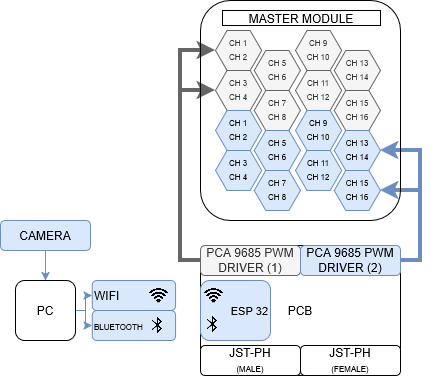
\includegraphics[width=2.4in]{figures/SOFIA_DIAGRAM}
		\caption{Block diagram describing SOFIA components and connections.}
		\label{fig1}
	\end{figure}
	
	\subsection{ESP32-C3 Technical Analysis}
	\linelabel{ln:spec-esp-intro}The main technical specifications of the ESP32-C3 microcontroller are presented in Table~\ref{tab:esp32_specs}.
	
	\begin{table}[!t]
		\centering
		\caption{ESP32-C3 Main Specifications and Datasheet Verification \cite{esp32c3}}
		\label{tab:esp32_specs}
		\scriptsize
		
		\setlength{\tabcolsep}{2pt}
		\renewcommand{\arraystretch}{1.1}
		
		\begin{tabularx}{\columnwidth}{@{}P{1.6cm} P{1.5cm} P{2.1cm} X X@{}}
			\toprule
			\textbf{Parameter} & \textbf{Value} & \textbf{Source (Doc / Ver / Pg)} & \textbf{Justification} & \textbf{Verification} \\
			\midrule
			
			Supply Voltage & 
			3.0--3.6 V & 
			ESP32-C3 Datasheet v2.4, p. 18 & 
			Match system main power operating limits & 
			Requires regulated 3.3 V supply \\
			
			Wi-Fi & 
			802.11 b/g/n & 
			ESP32-C3 Datasheet v2.4, p. 2 & 
			Enable 2.4 GHz wireless transmission & 
			Complies; integrated 2.4 GHz subsystem \\
			
			Bluetooth & 
			BLE 5 & 
			ESP32-C3 Datasheet v2.4, p. 2 & 
			Support low-energy configuration and monitoring & 
			Complies; Bluetooth LE 5.0 supported \\
			
			Logic Level & 
			3.3 V GPIO & 
			ESP32-C3 Datasheet v2.4, p. 19 & 
			Ensure digital signal levels meet peripheral logic thresholds & 
			5 V logic cannot be applied directly without level shifting \\
			
			Boot Pins & 
			GPIO2, 8, 9 & 
			ESP32-C3 Datasheet v2.4, p. 12 & 
			Prevent unintended strapping state selection during power-up & 
			PCB design hardware strapping verification required \\
			
			Temperature & 
			Up to 105 $^\circ$C & 
			ESP32-C3 Datasheet v2.4, p. 18 & 
			Ensure reliable continuous execution under thermal load & 
			Suitable for industrial and laboratory operating environments \\
			
			\bottomrule
		\end{tabularx}
	\end{table}
	
	% Source: ESP32-C3 Datasheet, Espressif Systems. (reference included in table caption)
	
	
	\subsection{PCA9685 Technical Analysis}
	\linelabel{ln:spec-pca-intro}The specifications of the PCA9685 PWM driver are summarized in Table~\ref{tab:pca9685_specs}.
	
	\begin{table}[!t]
		\centering
		\caption{PCA9685 Main Specifications and Datasheet Verification \cite{pca9685}}
		\label{tab:pca9685_specs}
		\scriptsize
		
		\setlength{\tabcolsep}{2pt}
		\renewcommand{\arraystretch}{1.1}
		
		\begin{tabularx}{\columnwidth}{@{}P{1.5cm} P{1.4cm} P{2.2cm} X X@{}}
			\toprule
			\textbf{Parameter} & \textbf{Value} & \textbf{Source (Doc / Ver / Pg)} & \textbf{Justification} & \textbf{Verification} \\
			\midrule
			
			Channels & 
			16 PWM & 
			PCA9685 Datasheet Rev. 7.5, p. 1 & 
			Control multiple servos with minimal MCU pin overhead & 
			Two devices provide 32 outputs \\
			
			Resolution & 
			12 bits & 
			PCA9685 Datasheet Rev. 7.5, p. 1 & 
			High-precision duty-cycle control for smooth motion & 
			Complies; 4096-step resolution \\
			
			Interface & 
			$\text{I}^2\text{C}$ FM+ & 
			PCA9685 Datasheet Rev. 7.5, p. 1 & 
			Standardized serial bus compatible with host controller & 
			Compatible with ESP32-C3 $\text{I}^2\text{C}$ peripheral \\
			
			Supply Voltage & 
			2.3--5.5 V & 
			PCA9685 Datasheet Rev. 7.5, p. 52 & 
			Operate on standard 3.3 V logic power rail & 
			Uses 3.3 V logic power supply \\
			
			PWM Frequency & 
			24--1526 Hz & 
			PCA9685 Datasheet Rev. 7.5, p. 1 & 
			Match standard RC servo control signal requirements & 
			Configured to 50 Hz output frequency \\
			
			Addressing & 
			Up to 62 ICs & 
			PCA9685 Datasheet Rev. 7.5, p. 12 & 
			Support unique addressing for cascading multiple ICs & 
			Configured with distinct fixed addresses (0x40 and 0x41) \\
			
			\bottomrule
		\end{tabularx}
	\end{table}
	
	% Source: PCA9685 Datasheet, NXP. (reference included in table caption)
	
	
	\subsection{MG90S Servo Technical Analysis}
	\linelabel{ln:spec-mg-intro}The nominal operating characteristics of the MG90S servomotor are presented in Table~\ref{tab:mg90s_specs}.
	
	\begin{table}[!t]
		\centering
		\caption{MG90S Main Specifications and Datasheet Verification \cite{mg90s}}
		\label{tab:mg90s_specs}
		\scriptsize
		
		\setlength{\tabcolsep}{2pt}
		\renewcommand{\arraystretch}{1.1}
		
		\begin{tabularx}{\columnwidth}{@{}P{1.5cm} P{1.7cm} P{2.cm} P{1.5cm} X@{}}
			\toprule
			\textbf{Parameter} & \textbf{Value} & \textbf{Source (Doc / Ver / Pg)} & \textbf{Justification} & \textbf{Verification} \\
			\midrule
			
			Voltage & 
			4.8--6.0 V & 
			TowerPro MG90S documentation, p. 1 & 
			Match system 5 V main power & 
			Compatible with 5 V \\
			
			Torque & 
			1.8 kgf$\cdot$cm at 4.8 V; \newline 2.2 kgf$\cdot$cm at 6.0 V & 
			TowerPro MG90S documentation, p. 1 & 
			Provide required joint actuation torque under load & 
			1.88 kgf$\cdot$cm available at 5.0 V; validation required \\
			
			Speed & 
			0.10 s/60$^\circ$ at 4.8 V; \newline 0.08 s/60$^\circ$ at 6.0 V & 
			TowerPro MG90S documentation, p. 1 & 
			Ensure joint angular velocity meets dynamic motion profile & 
			Reference value; complies for target control loop speed \\
			
			Mass & 
			13.4 g & 
			TowerPro MG90S documentation, p. 1 & 
			Minimize total end-effector and leg inertia & 
			Must be considered in structural mass budget and CAD model \\
			
			PWM Frequency & 
			50 Hz & 
			TowerPro MG90S documentation, p. 1 & 
			Standard RC servo control signal frame timing (20 ms period) & 
			Compatible with PCA9685 PWM output driver \\
			
			Stall Current & 
			Not reported & 
			TowerPro MG90S documentation, p. 1 & 
			Sizing power supply current limits for worst-case loading & 
			Not specified in datasheet; physical current measurement required \\
			
			\bottomrule
		\end{tabularx}
	\end{table}
	
	% Source: TowerPro MG90S documentation. (reference included in table caption)
	
	
	\subsection{Checklist Verification}
	\linelabel{ln:verification-intro}The preliminary component compatibility assessment is summarized in Table~\ref{tab:verification}.
	
	\begin{table}[!t]
		\centering
		\caption{Verification Summary}
		\label{tab:verification}
		\scriptsize
		
		\setlength{\tabcolsep}{2pt}
		\renewcommand{\arraystretch}{1.05}
		
		\begin{tabularx}{\columnwidth}{@{}P{2cm} P{1.7cm} Y@{}}
			\toprule
			Component & Status & Comment\\
			\midrule
			
			ESP32-C3 & 
			\status{Complies} & 
			Requires 3.3 V regulation and boot verification \\
			
			PCA9685 & 
			\status{Complies} & 
			Requires unique I2C addresses and 50 Hz configuration \\
			
			MG90S & 
			\status{Partial} & 
			Torque and current require validation \\
			
			\bottomrule
		\end{tabularx}
	\end{table}
	
	
	\subsection{RS-485 Logic-Level Compatibility}\label{sec:rs485_logic}
	
	To enable communication with an additional set of 16 SOFIA
	modules, the proposed architecture incorporates the
	MAX13487E TTL485-V2.0 transceiver module. The MAX13487E
	provides half-duplex RS-485 communication with automatic
	direction control, reducing the need for additional
	transmission-direction control signals \cite{max13487e}.
	
	According to the manufacturer's datasheet, the MAX13487E
	operates with a nominal 5 V supply, whereas the ESP32-C3
	uses 3.3 V GPIO logic \cite{max13487e,esp32c3}.
	A preliminary electrical test identified a receiver-output
	voltage of approximately 5.00 V at the TXD terminal of
	the TTL485-V2.0 module. This voltage exceeds the
	permitted input range of the ESP32-C3.
	
	\linelabel{ln:rs485-divider}To address this incompatibility, a resistive voltage
	divider was incorporated into the PCB schematic between
	the TTL485-V2.0 TXD output and the ESP32-C3 UART receive
	input. The divider consists of a 10 kOhm series resistor
	and an 18 kOhm resistor connected to ground, producing
	approximately 3.21 V from a nominal 5 V input.
	
	The ESP32-C3 UART transmit output remains directly
	connected to the TTL485-V2.0 RXD input, since the
	MAX13487E specifies a minimum logic-high input voltage
	of 2.0 V \cite{max13487e}.
	
	The voltage-divider circuit is included in the revised
	PCB schematic. Experimental verification of the
	assembled PCB remains pending.
	
	\subsection{Bill of Materials}
	\linelabel{ln:bom-intro}The components required for the SOFIA demonstrator,
	including mechanical parts, actuators, and electronic
	devices, are summarized in Table~\ref{tab:bom}.
	
	
	\begin{table}[!t]
		\centering
		\caption{SOFIA Demonstrator Bill of Materials (BOM) Summary}
		\label{tab:bom}
		\tiny
		
		\setlength{\tabcolsep}{1.5pt}
		\renewcommand{\arraystretch}{1.05}
		
		\begin{tabularx}{\columnwidth}{@{}P{0.8cm} P{2.0cm} P{0.5cm} P{0.5cm} P{2.4cm} P{1.1cm} P{0.8cm}@{}}
			\toprule
			\textbf{Item} & \textbf{Component} & \textbf{Qty / Unit} & \textbf{Qty / Sys} & \textbf{Technical Description} & \textbf{Manufacturer} & \textbf{Location} \\
			\midrule
			
			1 & Sofia003-P001-03 & 1 & 16 & Sofia Module Base & In-house (LabDST) & ITESO, MX \\
			2 & MG90S / SG90 Servo & 2 & 32 & Micro Servo Motor & Tower Pro & Hong Kong \\
			3 & Sofia003-E002-01 & 1 & 16 & Lower Joint Subassembly & In-house (LabDST) & ITESO, MX \\
			3.1/4.4 & Pro3 & 2 & 32 & Servo Horn & Tower Pro & Hong Kong \\
			3.2 & Sofia003-P004-02 & 1 & 16 & Lower Joint Support Left & In-house (LabDST) & ITESO, MX \\
			3.3 & Sofia003-P004-03 & 1 & 16 & Lower Joint Support Right & In-house (LabDST) & ITESO, MX \\
			3.4/3.5/ 4.3/7/8 & M2 Screws (various) & 10 & 160 & Servo Arm Screw ($M2 \times 10/12$ mm) & Walfront & Shenzhen, CN \\
			3.6 & Axis 1 ($9 \times 9$ mm) & 1 & 16 & Joint Shaft ($9\text{ mm} \times 9\text{ mm}$) & Mae & Local \\
			3.7 & Sofia003-P002-02 & 1 & 16 & Lower Joint Link & In-house (LabDST) & ITESO, MX \\
			4 & Sofia003-E003-01 & 1 & 16 & Upper Joint Subassembly & In-house (LabDST) & ITESO, MX \\
			4.1 & Sofia003-P005-01 & 1 & 16 & Upper Joint Support Left & In-house (LabDST) & ITESO, MX \\
			4.2 & Sofia003-P005-02 & 1 & 16 & Upper Joint Support Right & In-house (LabDST) & ITESO, MX \\
			5 & Sofia003-P008-01 & 1 & 16 & Sofia Top Module Linkage & In-house (LabDST) & ITESO, MX \\
			6 & Sofia003-P009-01 & 1 & 16 & Top Platform Support & In-house (LabDST) & ITESO, MX \\
			9 & Inser M3x5x4 & 1 & 16 & M3 Threaded Insert ($5 \times 4$ mm) & ZWMSSLL & Shenzhen, CN \\
			10 & Sofia003-P000-01 & 1 & 16 & Sofia Hexagonal Top Platform & In-house (LabDST) & ITESO, MX \\
			\midrule
			-- & ESP32-C3 SuperMini & -- & 1 & Central MCU (Wi-Fi/BLE telemetry) & Espressif & Shanghai, CN \\
			-- & PCA9685 Servo Driver & -- & 2 & 16-channel 12-bit $\text{I}^2\text{C}$ PWM driver board & NXP Semi & Eindhoven, NL \\
			-- & MAX13487E TTL485 & -- & 1 & Controller-side half-duplex RS-485 transceiver & Analog Devices & Wilmington, US \\
			-- & LED RGB & -- & 1 & System state status indicator LED & Mexbit & Local \\
			-- & JST-PH Male & -- & 1 & High-current power PCB header & JTAREA & Local \\
			-- & JST-PH Female & -- & 1 & High-current power harness plug & JTAREA & Local \\
			-- & R1--R5 (Resistors) & -- & 5 & RGB LED: 470 $\Omega$ (R1), 330 $\Omega$ (R2--R3); RS-485 divider: 10 k$\Omega$ (R4), 18 k$\Omega$ (R5) & Mexbit & Local \\
			
			\bottomrule
		\end{tabularx}
	\end{table}
	
	\subsection{Justification of Technological Selection}
	
	\begin{table}[!t]
		\centering
		\caption{Trade-Off Analysis for Actuation}
		\label{tab:alt_actuation}
		\scriptsize
		\setlength{\tabcolsep}{3pt}
		\renewcommand{\arraystretch}{1.1}
		\begin{tabularx}{\columnwidth}{@{}l c c X c@{}}
			\toprule
			\textbf{Alternative} & \textbf{Torque} & \textbf{Mass} & \textbf{Key Limitation / Feature} & \textbf{Sel.} \\
			\midrule
			MG996R \cite{mg996r} & High & $55\text{ g}$ & Excessive size and current draw & \\
			SG90 \cite{sg90} & Low & $9\text{ g}$ & Fragile nylon gears under load & \\
			\textbf{MG90S \cite{mg90s}*} & Medium & $13.4\text{ g}$ & Metal gears; optimal torque/size & \checkmark \\
			\bottomrule
		\end{tabularx}
	\end{table}
	
	\begin{table}[!t]
		\centering
		\caption{Trade-Off Analysis for PWM Expansion}
		\label{tab:alt_pwm}
		\scriptsize
		\setlength{\tabcolsep}{3pt}
		\renewcommand{\arraystretch}{1.1}
		\begin{tabularx}{\columnwidth}{@{}l c X c@{}}
			\toprule
			\textbf{Alternative} & \textbf{Channels} & \textbf{Key Limitation / Feature} & \textbf{Sel.} \\
			\midrule
			Software PWM \cite{esp32c3} & Limited & High MCU timer overhead; Limited GPIO & \\
			Auxiliary MCU \cite{stm32f4} & Flexible & Requires custom firmware and PCB space & \\
			\textbf{PCA9685 \cite{pca9685}*} & 16 & Hardware 12-bit PWM over $\text{I}^2\text{C}$ bus & \checkmark \\
			\bottomrule
		\end{tabularx}
	\end{table}
	
	\begin{table}[!t]
		\centering
		\caption{Trade-Off Analysis for Main Controller}
		\label{tab:alt_processing}
		\scriptsize
		\setlength{\tabcolsep}{3pt}
		\renewcommand{\arraystretch}{1.1}
		\begin{tabularx}{\columnwidth}{@{}l c X c@{}}
			\toprule
			\textbf{Alternative} & \textbf{Telemetry} & \textbf{Key Limitation / Feature} & \textbf{Sel.} \\
			\midrule
			Arduino Nano \cite{atmega328p} & None & 8-bit AVR; lacks integrated wireless & \\
			STM32F4 Core \cite{stm32f4} & External & High compute; larger board area & \\
			\textbf{ESP32-C3 SuperMini \cite{esp32c3}*} & Native & 32-bit RISC-V with Wi-Fi/BLE & \checkmark \\
			\bottomrule
		\end{tabularx}
	\end{table}
	
	\begin{table}[!t]
		\centering
		\caption{Trade-Off Analysis for Inter-Module Communication}
		\label{tab:alt_comm}
		\scriptsize
		\setlength{\tabcolsep}{3pt}
		\renewcommand{\arraystretch}{1.1}
		\begin{tabularx}{\columnwidth}{@{}l c X c@{}}
			\toprule
			\textbf{Alternative} & \textbf{Topology} & \textbf{Key Limitation / Feature} & \textbf{Sel.} \\
			\midrule
			Direct UART \cite{esp32c3} & Point-to-Point & Poor multi-drop scalability & \\
			CAN Bus \cite{sn65hvd230} & Multi-drop & High protocol/driver complexity & \\
			\textbf{RS-485 (MAX13487E) \cite{max13487e}*} & Multi-drop & Differential noise immunity + auto direction & \checkmark \\
			\bottomrule
		\end{tabularx}
	\end{table}
	
	\linelabel{ln:sel}The technological
	architecture was selected according to the functional and scalability
	requirements of the SOFIA demonstrator. 
	\linelabel{ln:sel-mg}MG90S servomotors as stated in Table~\ref{tab:alt_actuation} were selected to provide controlled angular positioning for each degree of freedom,
	while two PCA9685 drivers as stated in Table~\ref{tab:alt_pwm} were selected to  provide the 32 PWM channels required by the system through a shared I2C bus. The ESP32-C3 SuperMini as stated in Table~\ref{tab:alt_processing} was selected as the main controller due to its integrated wireless connectivity and support for the required communication interfaces. \linelabel{ln:sel-rs485}Finally, RS-485 as stated in Table~\ref{tab:alt_comm} was selected for inter-module communication because its differential and multi-node architecture supports the future connection of multiple
	SOFIA modules.
	
	\subsection{Servo Mechanical Time Constant Estimation}
	\linelabel{ln:servo-model}The first-order dynamic model for the angular position response $\theta(t)$ to a step input is defined by:
	\begin{equation}
		\theta(t) = \theta_f + (\theta_0 - \theta_f) e^{-t / \tau_m}
		\label{eq:servo_first_order}
	\end{equation}
	where $\theta_0$ represents the initial angular position, $\theta_f$ denotes the commanded step target angle, and $\tau_m$ is the servo mechanical time constant. 
	
	\linelabel{ln:servo-protocol}To characterize $\tau_m$, no-load step responses of $60^\circ$ will be applied while measuring the transient velocity profile. As noted in Table~\ref{tab:mg90s_specs}, the manufacturer datasheet \cite{mg90s} lists nominal angular speed ($0.10\text{ s}/60^\circ$ at $4.8\text{ V}$ and $0.08\text{ s}/60^\circ$ at $6.0\text{ V}$) but omits the explicit value for $\tau_m$, necessitating experimental identification.
	
	\section{Design and Implementation of the Technological Solution}
	\label{sec:design}
	
	Figure~\ref{fig2} \linelabel{ln:sim}shows the simulated response of the sixteen-module SOFIA structure while tracking the moving point. The sequence illustrates each module reorientation at different instants, where each module adjusts its two rotational degrees of freedom to maintain alignment with  reference position.
	
	\begin{figure}[!t]
		\centering
		\subfloat[Step 1]{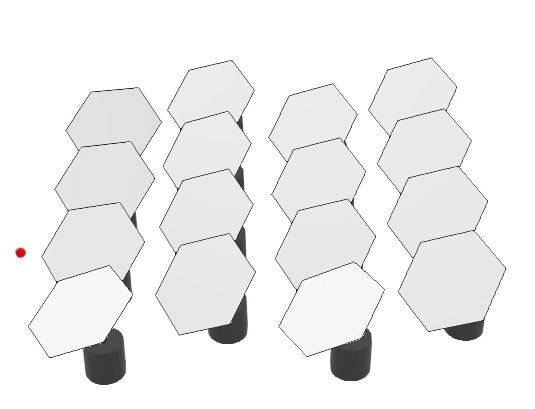
\includegraphics[width=1.1in]{figures/Sim_a}}
		\hfil
		\subfloat[Step 2]{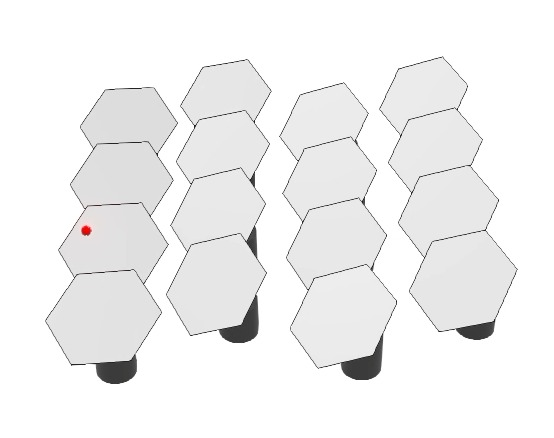
\includegraphics[width=1.1in]{figures/Sim_b}}
		\hfil
		\subfloat[Step 3]{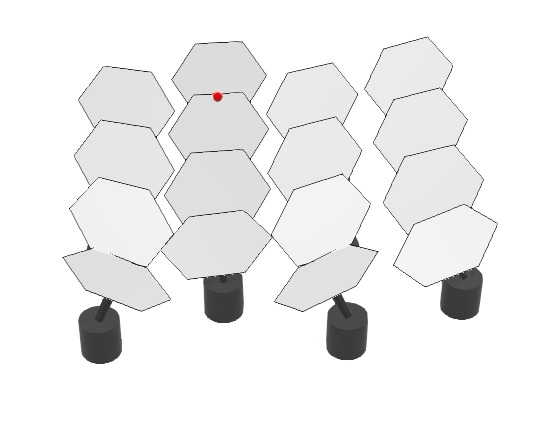
\includegraphics[width=1.1in]{figures/Sim_c}}
		\hfil
		\subfloat[Step 4]{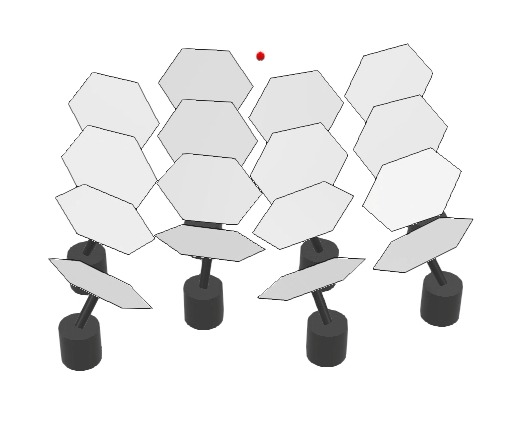
\includegraphics[width=1.1in]{figures/Sim_d}}
		\hfil
		\subfloat[Step 5]{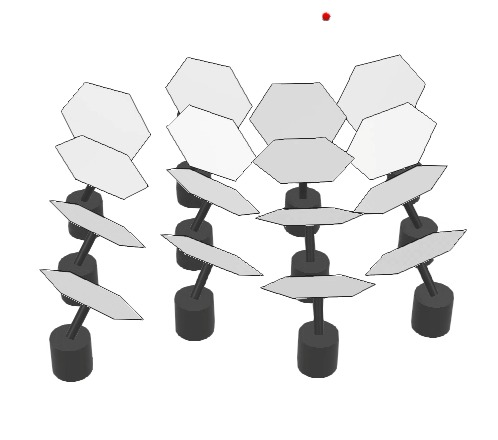
\includegraphics[width=1.1in]{figures/Sim_e}}
		\hfil
		\subfloat[Step 6]{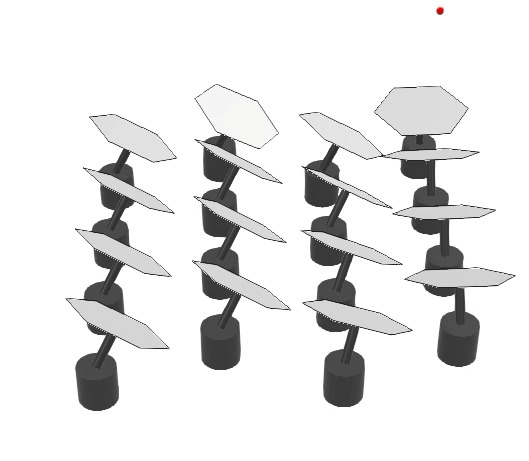
\includegraphics[width=1.1in]{figures/Sim_f}}
		\caption{Simulation of the SOFIA module tracking a moving reference point using inverse kinematics.}
		\label{fig2}
	\end{figure}
	
	Algorithm~\ref{alg:sofia_tracking} \linelabel{ln:alg}summarizes the inverse kinematics and smoothing strategy used by each SOFIA module to orient its platform toward the moving target.
	
	\begin{algorithm}[!t]
		\caption{SOFIA module target tracking control}
		\label{alg:sofia_tracking}
		
		
		\begin{algorithmic}[1]
			
			\Require Target position $\mathbf{p}$, module base position $\mathbf{r}_{0,2}$, joint limits $[q_{1\min}, q_{1\max}]$ and $[q_{2\min}, q_{2\max}]$, EMA smoothing factor $\alpha \in (0, 1]$
			\Ensure Servo command angles $q_1, q_2$
			
			\State $\mathbf{v} \gets \mathbf{p} - \mathbf{r}_{0,2}$
			\State $\hat{\mathbf{r}}_{2,p} \gets \frac{\mathbf{v}}{\|\mathbf{v}\|} = [u_x, u_y, u_z]^\top$ 
			
			\State $q_1^* \gets \operatorname{atan2}(-u_y, u_z)$
			\State $q_2^* \gets \arcsin(u_x)$ 
			
			\State $q_1^* \gets \Call{ClampAngle}{q_1^*, q_{1\min}, q_{1\max}}$
			\State $q_2^* \gets \Call{ClampAngle}{q_2^*, q_{2\min}, q_{2\max}}$
			
			\State $q_1 \gets q_{1,\text{old}} + \alpha (q_1^* - q_{1,\text{old}})$ \Comment{First-order EMA low-pass filter update}
			\State $q_2 \gets q_{2,\text{old}} + \alpha (q_2^* - q_{2,\text{old}})$
			
			\State Apply $q_1, q_2$ to servo motors
			
			\State \Return $q_1, q_2$
			
		\end{algorithmic}
	\end{algorithm}
	
	\subsection{Computer Vision System Architecture}
	
	\linelabel{ln:intro-vis}The computer vision subsystem of SOFIA was developed to recognize human gestures in real time and translate them into discrete action labels. The system uses a webcam to capture the user's movements and processes the images through a modular Python application. Its main purpose is to provide a gesture-based interaction method that can later be connected to the robot's control and actuation systems.
	
	\linelabel{ln:explain-vis}The implementation combines OpenCV for image acquisition and visualization with MediaPipe Tasks for human pose and hand landmark detection. Two pretrained models are used: Pose Landmarker, which identifies 33 body landmarks for one person, and Hand Landmarker, which detects up to two hands with 21 landmarks each. This approach avoids the need to train a custom neural network for gesture classification, since the detected landmarks are processed using predefined geometric rules.
	
	\linelabel{ln:model-vis}The software follows a modular architecture organized within the \texttt{Vision/} directory. The \texttt{main.py} file manages camera capture, model execution, gesture evaluation, and real-time visualization. The \texttt{pose\_detector.py} and \texttt{hand\_detector.py} modules handle body and hand landmark detection, respectively. Gesture classification is implemented in \texttt{gesture\_detector.py}, supported by \texttt{geometry\_utils.py} for geometric calculations and \texttt{smoothing.py} for temporal stabilization. Additional modules define the connections used to visualize body and hand landmarks.
	
	\linelabel{ln:model-vis2}During execution, each frame is captured in BGR format and converted to RGB before being processed by MediaPipe. The detected body landmarks are smoothed using an Exponential Moving Average (EMA) filter to reduce fluctuations between consecutive frames. The system then calculates geometric features, including normalized distances, joint angles, and relative positions, to evaluate the conditions associated with each gesture. Hand landmarks are also analyzed to identify specific finger configurations required for some interactions.
	
	\linelabel{ln:model-vis3}The recognition system supports five gestures: INICIO (Start), FIN (End), RECARGAR (Reload), ESCUDO (Shield), and ATAQUE (Attack). INICIO and FIN are classified as dynamic gestures because they require a sequence of movements over time, while RECARGAR, ESCUDO, and ATAQUE are static gestures identified through specific body and hand configurations. Once a gesture satisfies its recognition conditions, the system displays the corresponding label alongside the detected landmarks and an approximate frames-per-second (FPS) indicator.
	
	\linelabel{ln:model-vis4}At the current development stage, the computer vision subsystem operates as an independent perception prototype. Although its output is designed to support SOFIA's human-robot interaction, direct communication with the ESP32-C3 controller and physical actuation of the robotic modules have not yet been experimentally verified.
	
	\subsection{Geometric Gesture Recognition}
	
	\linelabel{ln:Geo-ges-rec-intro}The gesture recognition system was designed to identify five predefined human gestures through geometric analysis of body and hand landmarks. Instead of training a custom classification model, the implementation uses deterministic rules based on normalized distances, joint angles, relative positions, and movement sequences. This approach allows each gesture to be defined through specific conditions while keeping the recognition process modular and interpretable.
	
	\linelabel{ln:Geo-ges-rec2}To reduce the influence of the user's distance from the camera, several geometric measurements are normalized using anatomical references, such as shoulder width and torso height. The normalized distance between two landmarks is calculated as:
	\begin{equation}
		D_{\text{norm}} = \frac{\sqrt{(x_A - x_B)^2 + (y_A - y_B)^2}}{d_{\text{ref}}}
	\end{equation}
	where $A$ and $B$ represent the selected landmarks, and $d_{\text{ref}}$ is the distance between two anatomical reference points.
	
	\linelabel{ln:Geo-ges-rec3}For gestures involving arm positioning, joint angles are calculated using three landmarks. The angle between two vectors, with the elbow as the central point, is defined as:
	\begin{equation}
		\theta = \cos^{-1}\left( \frac{\mathbf{u} \cdot \mathbf{v}}{\|\mathbf{u}\| \|\mathbf{v}\|} \right)
	\end{equation}
	\linelabel{ln:Geo-ges-rec4}These angles are calculated from the two-dimensional projection of the detected landmarks and are used to evaluate arm configurations.
	
	\linelabel{ln:Geo-ges-rec5}The five gestures are divided into two dynamic gestures and three static gestures, depending on whether recognition requires a movement sequence or a specific body configuration described in Table~\ref{tab:gesture_conditions}.
	
	\begin{table}[!t]
		\centering
		\caption{Summary of Gesture Recognition Conditions}
		\label{tab:gesture_conditions}
		\vspace{0.5em}
		\begin{tabularx}{\columnwidth}{@{}c l X@{}}
			\toprule
			\textbf{Gesture} & \textbf{Type} & \textbf{Main recognition conditions} \\
			\midrule
			INICIO & Dynamic & Three wrist-to-hip contacts within 3s \\
			FIN & Dynamic & One raised hand and two horizontal direction changes \\
			RECARGAR & Static & Wrists near shoulders, approximately vertical forearms, no two recognized pistol hands \\
			ESCUDO & Static & Crossed arms, wrists near opposite shoulders, elbow below shoulders \\
			ATAQUE & Static & Elbow angles of 35$^\circ$--125$^\circ$ and two pistol-shaped hands \\
			\bottomrule
		\end{tabularx}
	\end{table}
	
	\linelabel{ln:vision-evaluation}The system evaluates these conditions using the body landmarks estimated by MediaPipe Pose Landmarker and the finger landmarks provided by MediaPipe Hand Landmarker. The resulting geometric conditions are used to determine the recognized gesture, while temporal confirmation mechanisms are applied to improve the stability of static gesture classification.
	
	\subsection{Temporal Filtering and Gesture Validation}
	
	\linelabel{ln:val-intro}To improve the stability of gesture recognition, the computer vision subsystem incorporates temporal filtering and validation mechanisms. These techniques were introduced to reduce fluctuations in detected body landmarks, prevent unintended gesture activations, and distinguish between temporary movements and intentional user actions.
	
	\linelabel{ln:val-ema-math}An Exponential Moving Average (EMA) filter is applied to the body landmarks detected by MediaPipe Pose Landmarker. This filter reduces variations between consecutive frames by combining the current landmark coordinates with their previously filtered values. The smoothing process is defined as:
	\begin{equation}
		S_t = \alpha X_t + (1 - \alpha) S_{t-1}
	\end{equation}
	where $S_t$ represents the smoothed landmark coordinate at time $t$, $X_t$ is the current detected coordinate, $S_{t-1}$ is the previous smoothed value, and $\alpha$ is the smoothing coefficient. The implemented system uses $\alpha = 0.3$, resulting in:
	\begin{equation}
		S_t = 0.3 X_t + 0.7 S_{t-1}
	\end{equation}
	
	\linelabel{ln:val-ema-proc}This operation is applied independently to the $x$, $y$, and $z$ coordinates of each body landmark. The filtered coordinates are then used by the geometric recognition algorithms, while the original landmarks remain available for visualization. When no body pose is detected, the smoothing state is reset to avoid reusing outdated coordinates. The hand landmarks used for finger classification are processed separately, without a confirmed implementation of the same EMA filter.
	
	\linelabel{ln:val-static-confirm}In addition to spatial smoothing, the system implements temporal confirmation for static gestures. Instead of accepting a gesture immediately after its geometric conditions are satisfied, the algorithm maintains a counter of consecutive valid frames. A static gesture is confirmed when its conditions remain satisfied for five consecutive frames. If any frame fails the required conditions, the counter returns to zero. This mechanism is implemented through the \texttt{TemporalConfirmation} class and helps prevent brief or unstable landmark configurations from being interpreted as intentional gestures.
	
	\linelabel{ln:val-dyn-inicio}Dynamic gestures require a different validation strategy because their recognition depends on movement sequences rather than maintaining a fixed posture. For INICIO, the algorithm uses a state-based counter to track three consecutive hand-to-thigh contact events. Hysteresis is introduced through separate contact and separation thresholds of 0.35 and 0.42, respectively. This prevents a single sustained contact from generating multiple detections. The complete sequence must occur within three seconds; otherwise, the accumulated contact count is reset.
	
	\linelabel{ln:val-dyn-fin}For FIN, the system tracks the horizontal movement of one raised hand. After selecting the active hand, the algorithm evaluates changes in its horizontal position and ignores displacements smaller than 0.12 in normalized coordinates. The first significant displacement establishes the initial movement direction, and subsequent direction reversals are counted. FIN is recognized after two valid reversals. If the active hand is lowered before completing the sequence, the tracking state is reset.
	
	\linelabel{ln:val-priority}Finally, the subsystem establishes a gesture display priority to manage situations in which multiple recognition conditions are satisfied simultaneously. The priority order is ESCUDO, ATAQUE, RECARGAR, INICIO, and FIN. This determines which label is displayed when different gesture detectors produce positive results, although the internal tracking states of other gestures may continue updating.
	
	\linelabel{ln:val-summary}Together, these mechanisms provide a structured approach to gesture stabilization and temporal validation. EMA filtering addresses frame-to-frame variations in body landmark positions, consecutive-frame confirmation reduces temporary static detections, and movement tracking allows dynamic gestures to be recognized through defined sequences. Although these techniques were functionally tested during development, their quantitative impact on recognition accuracy and response time has not yet been established through a complete experimental evaluation.
	
	\subsection{Integration Challenges and Design Refinements}
	
	\linelabel{ln:chal-intro}During the development of SOFIA's computer vision subsystem, several challenges were identified related to landmark stability, gesture recognition, software compatibility, and similarities between body configurations. These issues led to modifications in the recognition algorithms and software architecture to improve the functionality and usability of the prototype.
	
	\linelabel{ln:chal-mediapipe}One of the first challenges involved the compatibility and handling of MediaPipe detection results. The implementation uses the MediaPipe Tasks API for body and hand landmark estimation. During testing, the application encountered an \texttt{AttributeError} when the user temporarily disappeared from the camera's field of view. This occurred because the gesture detection module attempted to access pose landmarks when no valid detection was available. The issue was corrected by introducing validation for missing landmark data before processing the results, allowing the application to continue operating when the user was no longer visible.
	
	\linelabel{ln:chal-fluctuation}Another challenge was the fluctuation of body landmark coordinates between consecutive frames. Small variations in detected joint positions could affect geometric comparisons, particularly when the measurements were close to predefined recognition thresholds. To address this, an Exponential Moving Average filter with a smoothing coefficient of 0.3 was incorporated into the body landmark processing stage. Temporal confirmation requiring five consecutive valid frames was also introduced for static gesture recognition. Subsequent functional tests showed that the gesture recognition system continued operating with these mechanisms, although their quantitative effect on false positives and recognition accuracy was not measured.
	
	\linelabel{ln:chal-recargar}Significant changes were also made to the RECARGAR gesture. The initial implementation treated RECARGAR as a dynamic movement in which both hands moved upward from a lower position toward the shoulders within a limited time interval. However, the gesture specifications were later revised to require two dynamic gestures and three static gestures. As a result, RECARGAR was redesigned as a static configuration involving bent arms and hands positioned near shoulder height. Early versions of this new approach produced unintended detections when the user raised their arms during other gestures. To improve discrimination, additional geometric conditions were defined, including wrist proximity to the shoulders, bounded vertical positioning, and approximately vertical forearm orientation.
	
	\linelabel{ln:chal-overlap}A related problem involved the similarity between RECARGAR and ATAQUE. Certain arm positions could satisfy the geometric conditions of both gestures, particularly when the hands were close to shoulder level. To address this overlap, the final classification logic was designed to prevent RECARGAR from being recognized when both hands were identified as forming pistols. This introduced an additional distinction based on hand landmarks rather than body geometry alone. However, the effectiveness of this modification has not yet been established through a complete evaluation of the final implementation.
	
	\linelabel{ln:chal-ataque-old}The ATAQUE gesture required a substantial redesign to improve its recognition and make the movement more comfortable for different body configurations. The original algorithm required the elbows to remain close to the torso and included a depth-based condition to identify the forward orientation of the wrists. During development, these restrictions made the gesture difficult to perform consistently. An intermediate version using a wider elbow angle range of 90$^\circ$ to 165$^\circ$ was also tested but did not produce the expected recognition behavior.
	
	\linelabel{ln:chal-ataque-new}The gesture was consequently redefined using an approximately W-shaped arm configuration, with elbow angles between 35$^\circ$ and 125$^\circ$ and both wrists positioned above their respective elbows. The depth restriction and the requirement to keep the elbows close to the torso were removed. Additionally, the hands were oriented outward rather than directly toward the camera, making the pistol-shaped finger configurations easier to observe. Qualitative testing of this revised gesture produced satisfactory recognition, although its performance across different users has not been quantitatively evaluated.
	
	\linelabel{ln:chal-software}Finally, software organization introduced additional integration challenges. During development, the computer vision files were reorganized into a dedicated \texttt{Vision/} directory to improve modularity and maintainability. This change produced an import error involving the local performance metrics module. The import path was corrected, and successful execution of the application was subsequently confirmed. The final availability and integration of the metrics logging files, however, still require verification.
	
	\subsection{PCB Design and Electronic Integration}
	\label{subsec:pcb_design}
	
	A custom printed circuit board (PCB) was designed
	to integrate the electronic control and communication
	modules of the SOFIA kinetic surface. The PCB
	functions as a carrier board, providing mechanical
	mounting and electrical interconnections for the
	ESP32-C3 SuperMini microcontroller, two PCA9685
	PWM driver modules, and the MAX13487E RS-485
	transceiver interfaces.
	
	The ESP32-C3 serves as the main controller,
	communicating with the PCA9685 modules through
	the I2C interface. Each PCA9685 provides 16 PWM
	channels, allowing the proposed architecture to
	control up to 32 servomotors. The RS-485 interfaces
	enable differential serial communication with
	additional SOFIA modules.
	
	The PCB incorporates JST-PH connectors with a
	2.0 mm pitch, selected to meet the physical
	interconnection requirements of the system.
	Dedicated mounting positions and electrical
	connections are also provided for the control
	modules, communication interfaces, and an RGB LED.
	
	To address the logic-level incompatibility between
	the 5 V MAX13487E transceiver and the 3.3 V
	ESP32-C3 microcontroller, a resistive voltage
	divider was incorporated into the PCB schematic.
	The circuit consists of a 10 kOhm resistor (R4)
	and an 18 kOhm resistor (R5), reducing a nominal
	5 V receiver-output signal to approximately
	3.21 V at the ESP32-C3 UART input. The electrical
	compatibility analysis is detailed in the
	RS-485 Logic-Level Compatibility subsection
	of Materials and Methods.
	
	The electronic schematic is presented in
	Fig.~\ref{fig:sofia_schematic}, illustrating the
	connections between the microcontroller, PWM
	drivers, communication interfaces, and peripheral
	components.
	
	\begin{figure*}[!t]
		\centering
		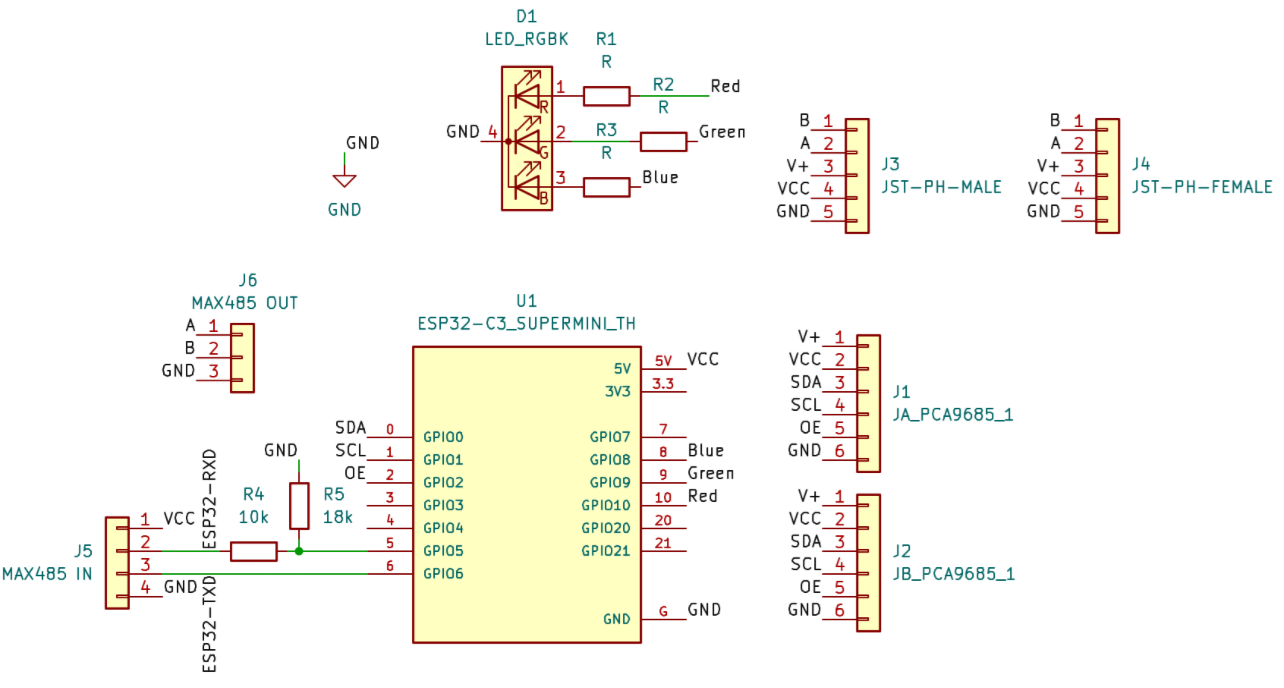
\includegraphics[width=0.95\textwidth]{figures/sofia_pcb_schematic.png}
		\caption{Electronic schematic of the SOFIA carrier PCB,
			showing the ESP32-C3 microcontroller, PCA9685 PWM
			driver interfaces, MAX13487E RS-485 connections,
			and peripheral circuitry.}
		\label{fig:sofia_schematic}
	\end{figure*}
	
	Based on the electronic schematic, a two-layer PCB
	layout was developed to organize component
	placement and signal routing. The resulting
	design, shown in Fig.~\ref{fig:sofia_pcb},
	provides a compact integration platform for
	the electronic modules and their connections.
	
	\begin{figure}[!t]
		\centering
		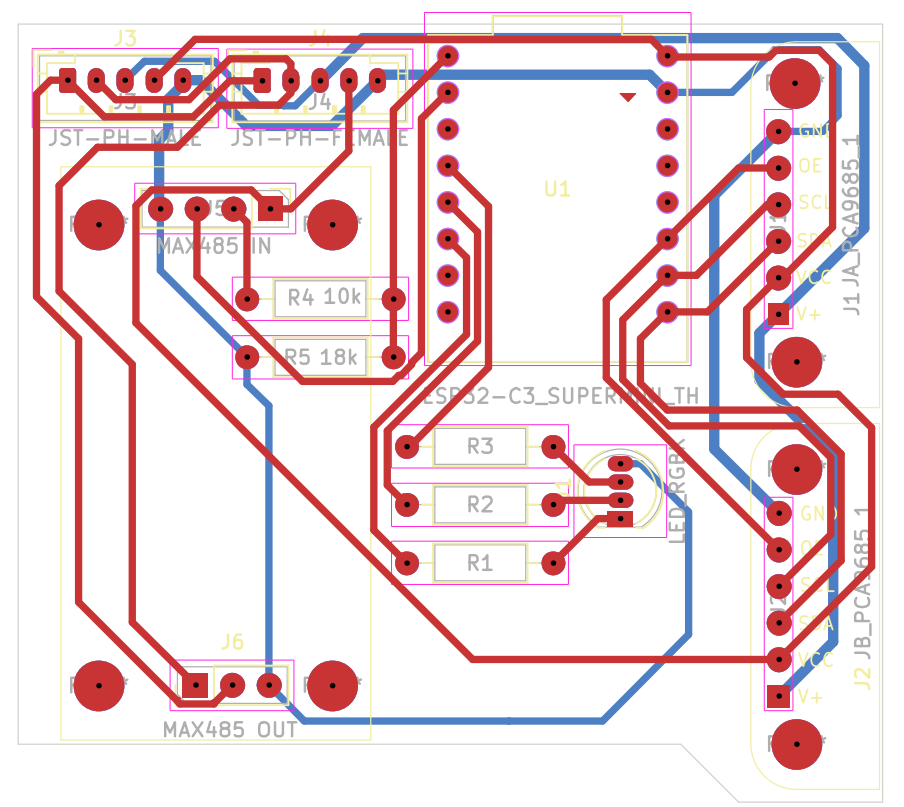
\includegraphics[width=\columnwidth]{figures/sofia_pcb.png}
		\caption{Completed two-layer PCB layout developed for the SOFIA electronic control system.}
		\label{fig:sofia_pcb}
	\end{figure}
	
	The PCB schematic and layout have been completed
	and are ready for the manufacturing stage.
	However, fabrication, assembly, and experimental
	validation of the PCB remain pending.
	
	
	
	\section{Results}
	\label{sec:results}
	
	\subsection{Experimental Setup}
	
	\subsection{Servomotor Dynamic Response}
	
	\subsection{Time Constant Estimation}
	
	\subsection{Functional Validation of the Vision Subsystem}
	
	\linelabel{ln:res-func-intro}The computer vision subsystem was tested through real-time webcam experiments to verify its ability to recognize the five predefined gestures. The tests focused on body and hand landmark detection, geometric gesture classification, and temporal validation.
	
	\linelabel{ln:vision-vis}The system successfully captured and processed video frames using OpenCV and MediaPipe, displaying the detected landmarks, recognized gesture labels, and approximate FPS in real time.
	
	\linelabel{ln:vision-func-tests}Functional tests confirmed the recognition of INICIO through three consecutive hand-to-thigh movements and FIN through two horizontal direction changes of a raised hand. For static gestures, ESCUDO was recognized through crossed-arm positioning, RECARGAR through the defined arm configuration near shoulder height, and ATAQUE through the combination of W-shaped arms and two pistol-shaped hands.
	
	\linelabel{ln:vision-func-ema}The implementation of EMA filtering and five-frame temporal confirmation maintained the functionality of the recognition system while providing mechanisms to reduce unstable detections. Additionally, the final adjustments to RECARGAR and ATAQUE were verified, confirming that the updated gesture definitions could be recognized during functional testing.
	
	\linelabel{ln:vision-func-summary}These results demonstrate the functional operation of the five-gesture recognition subsystem as an independent software prototype. However, recognition accuracy, average response time, and robustness under different environmental conditions still require quantitative evaluation.
	
	\subsection{Gesture Recognition Performance Evaluation}
	
	\linelabel{ln:res-vision-intro}Preliminary performance tests were conducted to evaluate gesture recognition and identify classification errors. These tests recorded the expected gesture, detected gesture, response time, and instantaneous frames per second (FPS).
	
	\linelabel{ln:vision-escudo}During the initial evaluation of ESCUDO, four attempts were recorded. Two were correctly classified, while the other two were incorrectly identified as RECARGAR.
	
	\begin{table}[!t]
		\centering
		\caption{Preliminary Performance Evaluation for ESCUDO Gesture}
		\label{tab:escudo_performance}
		\scriptsize
		\setlength{\tabcolsep}{3pt}
		\renewcommand{\arraystretch}{1.1}
		\begin{tabularx}{\columnwidth}{@{}l c c c c@{}}
			\toprule
			\textbf{Attempt} & \textbf{Expected} & \textbf{Detected} & \textbf{Time (ms)} & \textbf{FPS} \\
			\midrule
			Initial & ESCUDO & RECARGAR & 1841.65 & 26.62 \\
			1       & ESCUDO & ESCUDO   & 2072.08 & 21.95 \\
			2       & ESCUDO & ESCUDO   & 2306.67 & 20.27 \\
			3       & ESCUDO & RECARGAR & 2410.98 & 27.05 \\
			\bottomrule
		\end{tabularx}
	\end{table}
	
	\linelabel{ln:vision-overlap}These preliminary measurements helped identify overlapping recognition conditions between gestures, leading to refinements in the geometric classification rules.
	
	\linelabel{ln-vision-latency}The recorded response times included user reaction and gesture execution, as well as software processing. Therefore, they do not represent the algorithm's computational latency.
	
	\linelabel{ln:vision-adjustments}Following these observations, the recognition conditions for RECARGAR and ATAQUE were adjusted and their final functionality was verified. However, the preliminary measurements correspond to an earlier implementation and cannot be used to calculate the final system's accuracy.
	
	\section{Discussion}
	\label{sec:discussion}
	
	\section{Conclusions}
	\label{sec:conclusions}
	
	
	
	\balance
	
	\bibliographystyle{IEEEtran}
	\bibliography{bibliography}
	
\end{document}